\documentclass[aspectratio=43]{beamer}
\usetheme{CleanEasy}

\usepackage{amsmath}
\usepackage{amssymb}
\usepackage{booktabs}
\usepackage{graphicx}
\usepackage{tikz}
\usetikzlibrary{positioning,arrows.meta,shapes,calc}

\title{Group 23}
\subtitle{Risk-Averse Multi-Agent RL via Distribution Learning}
\date{\today}

\begin{document}

\begin{frame}
\titlepage
\end{frame}

% ==================================================
% Slide 1: The Problem
% ==================================================
\begin{frame}{The Problem}
\begin{center}
\textbf{Standard MARL optimizes expected reward}

\vspace{0.5em}

\textbf{Real-world systems need safety}
\end{center}

\vspace{0.3em}

\begin{center}
\includegraphics[width=0.5\textwidth]{figures/path_comparison.png}
\end{center}
\end{frame}

% ==================================================
% Slide 3: Prior Work on Risk-Averse RL
% ==================================================
\begin{frame}{Prior Work: Risk-Averse RL}
\begin{columns}[T]
\column{0.5\textwidth}
\textbf{Single-Agent Methods:}
\begin{itemize}
\item \textbf{Distributional RL}
    \begin{itemize}
    \item C51 (Bellemare et al., ICML 2017)
    \item QR-DQN (Dabney et al., AAAI 2018)
    \item Learn full return distribution
    \item Extract risk post-hoc
    \end{itemize}

\vspace{0.3em}

\item \textbf{Robust RL}
    \begin{itemize}
    \item Iyengar, Math. OR 2005
    \item Worst-case optimization
    \item Very conservative
    \end{itemize}

\vspace{0.3em}

\item \textbf{Mean-Variance}
    \begin{itemize}
    \item $\max E[R] - \lambda \text{Var}[R]$
    \item Hand-tune $\lambda$
    \end{itemize}
\end{itemize}

\column{0.5\textwidth}
\textbf{Multi-Agent Methods:}
\begin{itemize}
\item \textbf{RMIX / RiskQ}
    \begin{itemize}
    \item RMIX (Qiu et al., NeurIPS 2021)
    \item RiskQ (Shen et al., NeurIPS 2023)
    \item Value factorization + CVaR
    \item No equilibrium guarantees
    \end{itemize}

\vspace{0.3em}

\item \textbf{Reward Shaping}
    \begin{itemize}
    \item Manual per-environment
    \item Weak theory
    \end{itemize}
\end{itemize}

\vspace{1em}

\begin{center}
\textbf{\color{blue} Gap: No tractable risk-averse equilibrium for MARL!}
\end{center}
\end{columns}
\end{frame}

% ==================================================
% Slide 4: Risk Measures
% ==================================================
\begin{frame}{Risk Measures}
\begin{center}
\textbf{How to extract risk-adjusted value from distribution?}
\end{center}

\vspace{1em}

\begin{block}{Entropic Risk Measure}
\begin{equation*}
\rho_\tau(Z) = -\frac{1}{\tau} \log \mathbb{E}[\exp(-\tau Z)]
\end{equation*}
\vspace{0.5em}
\begin{itemize}
\item $\tau \to \infty$: Risk-neutral (expected value)
\item $\tau = 1.0$: Moderate risk-aversion
\item $\tau = 0.3$: High risk-aversion (pessimistic)
\end{itemize}
\end{block}
\end{frame}

% ==================================================
% Slide 5: How Do We Learn the Distribution?
% ==================================================
\begin{frame}{How Do We Learn the Distribution?}
\begin{columns}[T]
\column{0.5\textwidth}
\textbf{Standard RL:}
\begin{align*}
V(s) &= \mathbb{E}[\text{return}] \\
&= \text{scalar}
\end{align*}

\vspace{1em}
\textbf{Distributional RL:}
\begin{align*}
Z(s) &= \text{distribution over returns} \\
&= [p_1, p_2, \ldots, p_{51}]
\end{align*}

\column{0.5\textwidth}
\begin{center}
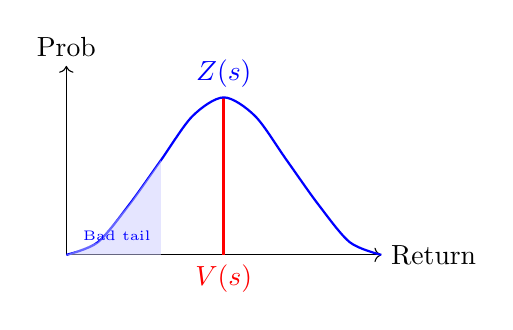
\begin{tikzpicture}[scale=0.8]
    % Axes
    \draw[->] (0,0) -- (5,0) node[right] {Return};
    \draw[->] (0,0) -- (0,3) node[above] {Prob};

    % Expected value (scalar)
    \draw[red,very thick] (2.5,0) -- (2.5,2.5);
    \node[red,below] at (2.5,0) {$V(s)$};

    % Distribution
    \draw[blue,thick,smooth] plot coordinates {
        (0,0) (0.5,0.2) (1,0.8) (1.5,1.5) (2,2.2)
        (2.5,2.5) (3,2.2) (3.5,1.5) (4,0.8) (4.5,0.2) (5,0)
    };
    \node[blue,above] at (2.5,2.5) {$Z(s)$};

    % Tail regions
    \fill[blue!20,opacity=0.5] (0,0) -- plot coordinates {
        (0,0) (0.5,0.2) (1,0.8) (1.5,1.5)
    } -- (1.5,0) -- cycle;
    \node[blue,font=\tiny] at (0.8,0.3) {Bad tail};
\end{tikzpicture}

\vspace{0.5em}
{\small Distribution reveals risk}
\end{center}
\end{columns}
\end{frame}

% ==================================================
% Slide 6: Bounded Rationality
% ==================================================
\begin{frame}{Bounded Rationality}

\begin{block}{Full PPO Loss}
\begin{equation*}
\mathcal{L}_{\text{total}} = \mathcal{L}_{\text{CLIP}} + c_1 \cdot \mathcal{L}_{\text{VF}} - \epsilon \cdot H(\pi)
\end{equation*}
\vspace{0.5em}

where $H(\pi) = -\sum_a \pi(a|s) \log \pi(a|s)$ (entropy)

\vspace{0.5em}
\begin{itemize}
\item $\epsilon = 0$: Deterministic (no exploration)
\item $\epsilon = 0.01$: Typical value (maintains exploration)
\item $\epsilon$ is \textbf{fixed} during training (not annealed)
\end{itemize}
\end{block}

\vspace{1em}

\begin{center}
\textbf{From behavioral economics: humans aren't perfectly rational}
\end{center}
\end{frame}

% ==================================================
% Slide 7: Theoretical Guarantee (Why Bounded Rationality?)
% ==================================================
\begin{frame}{Theoretical Guarantee: Why Bounded Rationality?}
\textbf{From Mazumdar et al. (2025):}

\vspace{0.5em}

\begin{block}{Theorem 3: Computational Tractability}
Risk-Averse QRE is \textbf{polynomial-time computable} via no-regret learning when:
\begin{equation*}
\epsilon_1 \epsilon_2 \geq \xi_1^* \xi_2^*
\end{equation*}
where $\epsilon_i$ = bounded rationality, $\xi_i^*$ = risk-aversion parameter
\end{block}

\vspace{0.5em}

\begin{itemize}
\item Without bounded rationality ($\epsilon = 0$): Nash equilibrium is PPAD-complete (intractable)
\item With bounded rationality ($\epsilon > 0$): Can use standard no-regret algorithms (tractable!)
\item \textbf{Note:} In practice, entropy regularization is already standard in RL. The paper provides \textbf{theoretical justification} for this design choice.
\end{itemize}
\end{frame}

% ==================================================
% Slide 8: Architecture Overview
% ==================================================
\begin{frame}{Distributional RQE-MAPPO Architecture}
\begin{center}
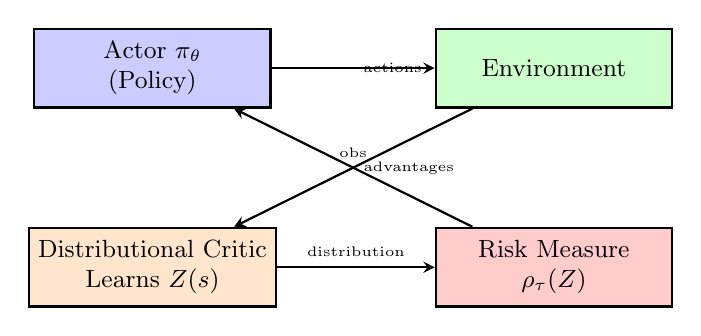
\begin{tikzpicture}[
    box/.style={rectangle,draw,minimum width=3cm,minimum height=1cm,align=center,font=\small,thick},
    arrow/.style={->,>=stealth,thick},
    node distance=1.5cm
]
    % Networks
    \node[box,fill=blue!20] (actor) {Actor $\pi_\theta$ \\ (Policy)};
    \node[box,fill=orange!20,below=of actor] (critic) {Distributional Critic \\ Learns $Z(s)$};
    \node[box,fill=red!20,right=2cm of critic] (risk) {Risk Measure \\ $\rho_\tau(Z)$};
    \node[box,fill=green!20,above=of risk] (env) {Environment};

    % Arrows
    \draw[arrow] (actor) -- (env) node[midway,right,font=\tiny] {actions};
    \draw[arrow] (env) -- (critic) node[midway,above,font=\tiny] {obs};
    \draw[arrow] (critic) -- (risk) node[midway,above,font=\tiny] {distribution};
    \draw[arrow] (risk) -- (actor) node[midway,right,font=\tiny] {advantages};
\end{tikzpicture}
\end{center}

\vspace{1em}

\textbf{Key Components:}
\begin{itemize}
\item \textbf{Distributional Critic}: Learns return distribution $Z(s)$
\item \textbf{Risk Measure}: Computes $V_\tau(s) = \rho_\tau(Z(s))$ for GAE
\item \textbf{Fixed Entropy}: $\epsilon \cdot H(\pi)$ for bounded rationality
\end{itemize}
\end{frame}

% ==================================================
% Slide 6: Training Objective
% ==================================================
\begin{frame}{Training Objective}
\begin{block}{1. Critic Loss (Distributional Bellman)}
\begin{equation*}
\mathcal{L}_{\text{critic}} = \text{CrossEntropy}(Z_{\text{current}}, Z_{\text{target}})
\end{equation*}

where $Z_{\text{target}} = \text{PROJECT}[r + \gamma Z(s')]$

\vspace{0.2em}
{\small KL divergence minimization between distributions}
\end{block}

\vspace{0.3em}

\begin{block}{2. Actor Loss (PPO + Entropy)}
\begin{equation*}
\mathcal{L}_{\text{actor}} = -\min(\text{ratio} \cdot \hat{A}, \text{clip}(\text{ratio}) \cdot \hat{A}) + \epsilon \cdot H(\pi)
\end{equation*}

\vspace{0.1em}

\textbf{Risk-adjusted advantages (GAE):}
\begin{align*}
\hat{A}_t &= \sum_{l=0}^{\infty} (\gamma \lambda)^l \delta_{t+l} \\
\delta_t &= r_t + \gamma V_\tau(s_{t+1}) - V_\tau(s_t) \\
V_\tau(s) &= \rho_\tau(Z(s)) = -\frac{1}{\tau} \log \mathbb{E}[\exp(-\tau Z(s))]
\end{align*}

\end{block}
\end{frame}

% ==================================================
% Slide 7: Environments
% ==================================================
\begin{frame}{Experimental Environments}
\begin{columns}[T]
\column{0.5\textwidth}
\textbf{1. Risky CartPole}
\begin{itemize}
\item Single-agent validation
\item Random wind gusts
\item Stochastic dynamics
\item Fast iteration ($<$30 min)
\end{itemize}

\vspace{1em}
\textbf{Expected:} Risk-averse agents survive longer under disturbances

\column{0.5\textwidth}
\textbf{2. Traffic Coordination (SUMO)}
\begin{itemize}
\item Multi-agent main domain
\item Intersection navigation
\item Safety-critical
\item Real-world relevance
\end{itemize}

\vspace{1em}
\textbf{Expected:} Lower collision rates with risk-aversion
\end{columns}

\vspace{2em}

\begin{center}
\textbf{Baselines:} Standard MAPPO ($\tau = \infty$), Reward-shaped MAPPO
\end{center}
\end{frame}

% ==================================================
% Slide 10: Experiments
% ==================================================
\begin{frame}{Experiments}
\textbf{Experiment 1: Comparison Against Risk-Averse Methods}

\vspace{0.3em}
{\small Compete against existing risk-averse MARL approaches:}

\vspace{0.3em}
\begin{itemize}
\item Standard MAPPO (risk-neutral baseline)
\item \textbf{C51-CVaR MAPPO} (Bellemare et al., 2017 + CVaR)
\item \textbf{RMIX} (Qiu et al., NeurIPS 2021)
\item \textbf{Mean-Variance MAPPO} (dual critic: $E[R] - \lambda \text{Var}[R]$)
\item \textbf{Reward-Shaped MAPPO} (manual safety penalties)
\item \textbf{RQE-MAPPO} (ours: entropic risk + bounded rationality)
\end{itemize}

\vspace{0.3em}
{\small Metrics: Mean return, Std dev, Collision rate, Worst 5\% returns}

\end{frame}

\begin{frame}
\textbf{Experiment 2: Risk-Reward Tradeoff}

\vspace{0.3em}
Sweep $\tau \in \{0.3, 0.5, 1.0, 2.0, 10.0\}$ for RQE

\vspace{0.3em}
Expected: Pareto curve (safety vs efficiency), single $\tau$ generalizes

\vspace{1em}

\textbf{Experiment 3: Ablation Study}

\vspace{0.3em}
\begin{itemize}
\item Risk only ($\tau < \infty$, $\epsilon = 0$) vs Rationality only ($\tau = \infty$, $\epsilon > 0$) vs Both
\end{itemize}

\vspace{0.3em}
Expected: Both components needed for best performance
\end{frame}

% ==================================================
% Slide 11: Implementation Status
% ==================================================
\begin{frame}{Implementation Status}
\begin{center}
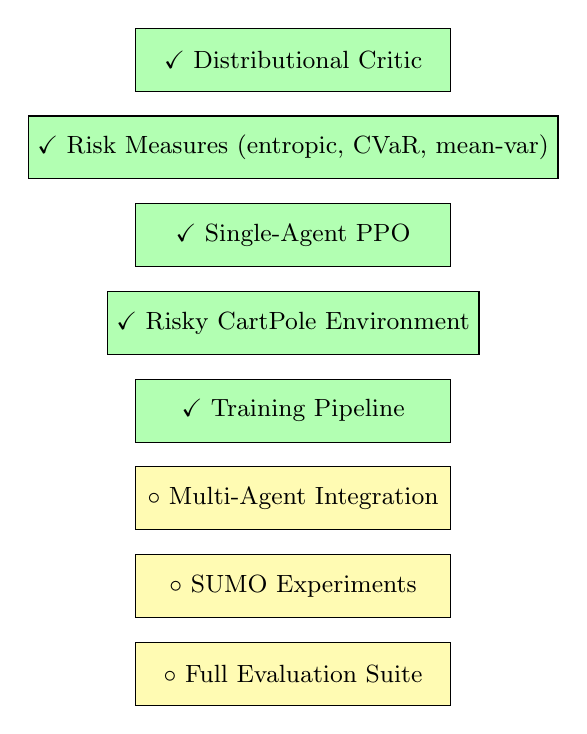
\begin{tikzpicture}[
    done/.style={rectangle,draw,fill=green!30,minimum width=4cm,minimum height=0.8cm,font=\small},
    todo/.style={rectangle,draw,fill=yellow!30,minimum width=4cm,minimum height=0.8cm,font=\small},
    node distance=0.3cm
]
    \node[done] (c1) {$\checkmark$ Distributional Critic};
    \node[done,below=of c1] (c2) {$\checkmark$ Risk Measures (entropic, CVaR, mean-var)};
    \node[done,below=of c2] (c3) {$\checkmark$ Single-Agent PPO};
    \node[done,below=of c3] (c4) {$\checkmark$ Risky CartPole Environment};
    \node[done,below=of c4] (c5) {$\checkmark$ Training Pipeline};
    \node[todo,below=of c5] (t1) {$\circ$ Multi-Agent Integration};
    \node[todo,below=of t1] (t2) {$\circ$ SUMO Experiments};
    \node[todo,below=of t2] (t3) {$\circ$ Full Evaluation Suite};
\end{tikzpicture}
\end{center}

\vspace{1em}

\textbf{Timeline:} 2-3 weeks to full experimental results
\end{frame}

% ==================================================
% Slide 13: Future Direction (Policy Interpolation)
% ==================================================
\begin{frame}{Future Direction: Policy Interpolation}
\textbf{Idea:} Train two policies, interpolate at inference time

\vspace{1em}

\begin{block}{Approach}
\textbf{Training:}
\begin{itemize}
\item Train risk-neutral policy: $\pi_{\text{neutral}}$ with $\tau = \infty$
\item Train risk-averse policy: $\pi_{\text{safe}}$ with $\tau = 0.3$
\end{itemize}

\vspace{0.5em}

\textbf{Inference (Policy Interpolation):}
\begin{equation*}
\pi_\alpha(a|s) = \alpha \cdot \pi_{\text{safe}}(a|s) + (1-\alpha) \cdot \pi_{\text{neutral}}(a|s)
\end{equation*}

\begin{itemize}
\item $\alpha = 1$: Fully risk-averse (safe, conservative)
\item $\alpha = 0.5$: Balanced behavior
\item $\alpha = 0$: Risk-neutral (efficient, aggressive)
\end{itemize}
\end{block}

\vspace{0.5em}

\begin{center}
\textbf{Benefit:} Tune safety-efficiency tradeoff \textit{without retraining}
\end{center}
\end{frame}

% ==================================================
% Slide 14: Questions
% ==================================================
\begin{frame}
\begin{center}
\Huge
\textbf{Questions?}
\end{center}
\end{frame}

\end{document}
